%! alt Regular hexagon ABCDEF with a point P inside it, joined to all six vertices. Triangles PAB, PBC and PCD carry their areas 7, 10 and 15. The triangles PAB, PCD and PEF on alternate sides are shaded. The sides AB, CD and EF are extended to form a large equilateral triangle around the hexagon; the distances from P to its three sides add up to its height, so the shaded triangles make half of the hexagon. The opposite sides BC and EF are parallel, so triangles PBC and PEF make a third of it, and the hexagon has area 72.
%! after_paragraph 1
%! scale 9/20
%! let s = 4*3**(1/4)
% The shared preamble of every Cevian figure. pipeline/figures turns these colours into theme-aware paint,
% and refuses any other colour, so draw only with them:
%   figink (lines and labels), figaux (construction lines), figaccent (the object the argument turns on),
%   figtint and figaccenttint (light fills).
\documentclass[border=1.5pt]{standalone}
\usepackage{tkz-euclide}
\definecolor{figink}{RGB}{0,0,0}
\definecolor{figaux}{RGB}{85,85,85}
\definecolor{figaccent}{RGB}{192,57,43}
\definecolor{figtint}{RGB}{221,221,221}
\definecolor{figaccenttint}{RGB}{245,213,208}
% tkz-euclide's defaults draw circles, compasses and marks in 50% grey and fill points with a tint.
\makeatletter
\def\tkz@otherlinecolor{figink}
\def\tkz@euc@circlecolor{figink}
\def\tkz@euc@compasscolor{figink}
\def\tkz@euc@mkcolor{figink}
\def\tkz@mk@fill{figink}
\def\tkz@euc@pointfillcolor{figink}
\makeatother
\tkzSetUpLine[color=figink,line width=.7pt]
\tkzSetUpArc[color=figink,line width=.7pt]
\tkzSetUpCompass[color=figink,line width=.5pt]
\tkzSetUpPoint[color=figink,fill=figink,size=3.1pt]
\tikzset{
  every picture/.style={line cap=round,line join=round,color=figink},
  circle style/.append style={color=figink,line width=.7pt},
  aux/.style={color=figaux,line width=.45pt,dash pattern=on 2.6pt off 2pt},
  key/.style={color=figaccent,line width=1pt},
  mk/.style={color=figink,line width=.5pt},
  lbl/.style={color=figink,inner sep=2.2pt},
  len/.style={color=figink,inner sep=1.5pt,font=\small},
}

\begin{document}
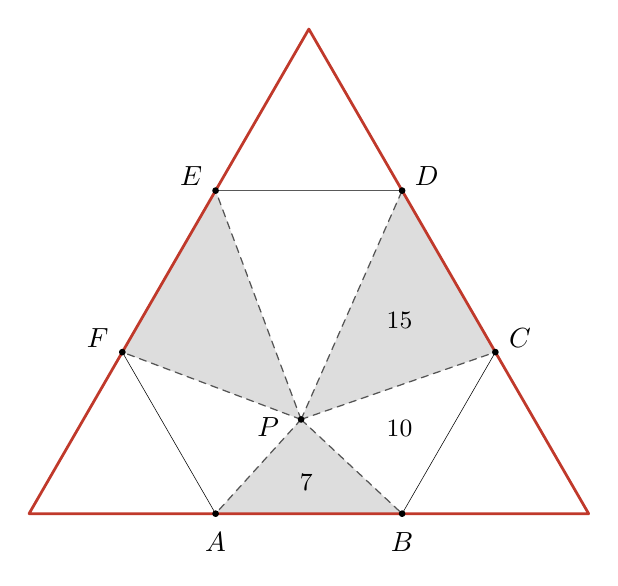
\begin{tikzpicture}
\tkzDefPoint(0.0,0.0){O} %! O = (0, 0)
\tkzDefPoint(-1.1844666,-2.0515564){A} %! A = polar(O, s, 240)
\tkzDefPoint(1.1844666,-2.0515564){B} %! B = polar(O, s, 300)
\tkzDefPoint(2.3689332,0.0){C} %! C = polar(O, s, 0)
\tkzDefPoint(1.1844666,2.0515564){D} %! D = polar(O, s, 60)
\tkzDefPoint(-1.1844666,2.0515564){E} %! E = polar(O, s, 120)
\tkzDefPoint(-2.3689332,0.000000000000000000000000000000000000000000000000010268932){F} %! F = polar(O, s, 180)
\tkzDefPoint(-0.098705551,-0.85481515){P} %! P = (-s/24, -5*sqrt(3)*s/24)
\tkzDefPoint(3.5533998,-2.0515564){X} %! X = shift(B, x(C), y(C))
\tkzDefPoint(0.0000000000000000000000000000000000000000000000000024054882,4.1031127){Y} %! Y = shift(D, x(E), y(E))
\tkzDefPoint(-3.5533998,-2.0515564){Z} %! Z = shift(F, x(A), y(A))
\tkzDefPoint(-1.1844666,-2.4115564){LA} %! LA = polar(A, 0.8, 270)
\tkzDefPoint(1.1844666,-2.4115564){LB} %! LB = polar(B, 0.8, 270)
\tkzDefPoint(2.6807024,0.18000000){LC} %! LC = polar(C, 0.8, 30)
\tkzDefPoint(1.4962358,2.2315564){LD} %! LD = polar(D, 0.8, 30)
\tkzDefPoint(-1.4962358,2.2315564){LE} %! LE = polar(E, 0.8, 150)
\tkzDefPoint(-2.6807024,0.18000000){LF} %! LF = polar(F, 0.8, 150)
\tkzDefPoint(-0.51524875,-0.95098172){LP} %! LP = polar(P, 0.95, 193)
\tkzDefPoint(-0.032901850,-1.6526426){T1} %! T1 = ((x(P) + x(A) + x(B))/3, (y(P) + y(A) + y(B))/3)
\tkzDefPoint(1.1515648,-0.96879050){T2} %! T2 = ((x(P) + x(B) + x(C))/3, (y(P) + y(B) + y(C))/3)
\tkzDefPoint(1.1515648,0.39891373){T3} %! T3 = ((x(P) + x(C) + x(D))/3, (y(P) + y(C) + y(D))/3)
%! fact area(P, A, B) == 7
%! fact area(P, B, C) == 10
%! fact area(P, C, D) == 15
%! fact area(A, B, C, D, E, F) == 72
%! fact area(P, B, C) + area(P, E, F) == area(A, B, C, D, E, F)/3
%! fact area(P, A, B) + area(P, C, D) + area(P, E, F) == area(A, B, C, D, E, F)/2
%! fact parallel(B, C, E, F)
%! fact collinear(X, A, B)
%! fact collinear(X, C, D)
%! fact collinear(Y, C, D)
%! fact collinear(Y, E, F)
%! fact collinear(Z, E, F)
%! fact collinear(Z, A, B)
%! fact dist(X, Y) == dist(Y, Z)
%! fact dist(Y, Z) == dist(Z, X)
\tkzFillPolygon[color=figtint](P,A,B)
\tkzFillPolygon[color=figtint](P,C,D)
\tkzFillPolygon[color=figtint](P,E,F)
\tkzDrawPolygon(A,B,C,D,E,F)
\tkzDrawPolygon[key](X,Y,Z)
\tkzDrawSegments[aux](P,A P,B P,C P,D P,E P,F)
\tkzDrawPoints(A,B,C,D,E,F,P)
\tkzLabelPoint[anchor=center,lbl](LA){$A$}
\tkzLabelPoint[anchor=center,lbl](LB){$B$}
\tkzLabelPoint[anchor=center,lbl](LC){$C$}
\tkzLabelPoint[anchor=center,lbl](LD){$D$}
\tkzLabelPoint[anchor=center,lbl](LE){$E$}
\tkzLabelPoint[anchor=center,lbl](LF){$F$}
\tkzLabelPoint[anchor=center,lbl](LP){$P$}
\tkzLabelPoint[anchor=center,len](T1){$7$}
\tkzLabelPoint[anchor=center,len](T2){$10$}
\tkzLabelPoint[anchor=center,len](T3){$15$}
\end{tikzpicture}
\end{document}
